\chapter{Numerical implementation}\label{chap:Numerical}

As with any physics problem that must be solved on a computer, there are aspects which must be treated using numerical approximations. Certain parts of the problem may take longer to evaluate than others, and occasionally one runs into problems of [machine] precision.

\section{Calculating the PES}
By far, the most time-intensive part of a microscopic fission calculation is the calculation of the PES. For this we use a pair of DFT solvers, HFODD \cite{Schunck2017} and HFBTHO \cite{Perez2017}. These programs solve the HFB equations in a basis of deformed harmonic oscillators. The solver HFBTHO is limited to shapes with axial symmetry, while HFODD allows for the breaking of any symmetry needed. However, since the major bottleneck of each of these programs involves constructing and then diagonalizing the matrix representing \verb|thing|, this flexibility drastically increases the time-to-solution.

The procedure is performed iteratively: First, a density ansatz is given (either by the user or by some simple means, such as a quick Woods-Saxon calculation). Then the energy density matrix is constructed, after which it is diagonalized and a new density matrix is calculated. The procedure then repeats for a fixed number of iterations, or until a predetermined convergence criterion is satisfied In HFODD, for instance, the default convergence criterion is for the difference between the total energy summed over all single-particle states and the total energy calculated by \verb|???| to be less than some user-defined value.

Certain parts of the procedure can be parallelized using shared-memory parallelism, such as QMULCM, which does what again?

On the positive side, the problem of calculating a PES is embarrassingly-parallel. So while an individual point in the PES may be difficult to compute, many points can be computed simultaneously. This does have its limitations; highly-deformed configurations may be very unstable because of reasons. One fix may sometimes be to use a nearby point which converged successfully as a seed function

\section{Calculating the collective inertia}
The partial derivatives from equation \ref{eq:mATDHFB-np} are computed using the Lagrange three-point formula:

\begin{equation}\label{eq:finite-diffs}
\left(\frac{\partial \mathcal{R}}{\partial q}\right)_{q=q_0} \approx 
    \frac{-\delta q'}{\delta q \left(\delta q + \delta q'\right)}\mathcal{R}(q_0-\delta q) + 
    \frac{\delta q - \delta q'}{\delta q \delta q'}\mathcal{R}(q_0) + 
    \frac{\delta q}{\delta q' \left(\delta q + \delta q'\right)}\mathcal{R}(q_0+\delta q')
\end{equation}

The accuracy and precision of the collective inertia $\mathcal{M}$ are therefore functions of the spacings $\delta q$ and $\delta q'$, and of $\mathcal{R}$. An accurate value of the collective inertia is especially important for computing half-lives, where there is an exponential dependence on $\mathcal{M}$.

\begin{figure}
	\centering
	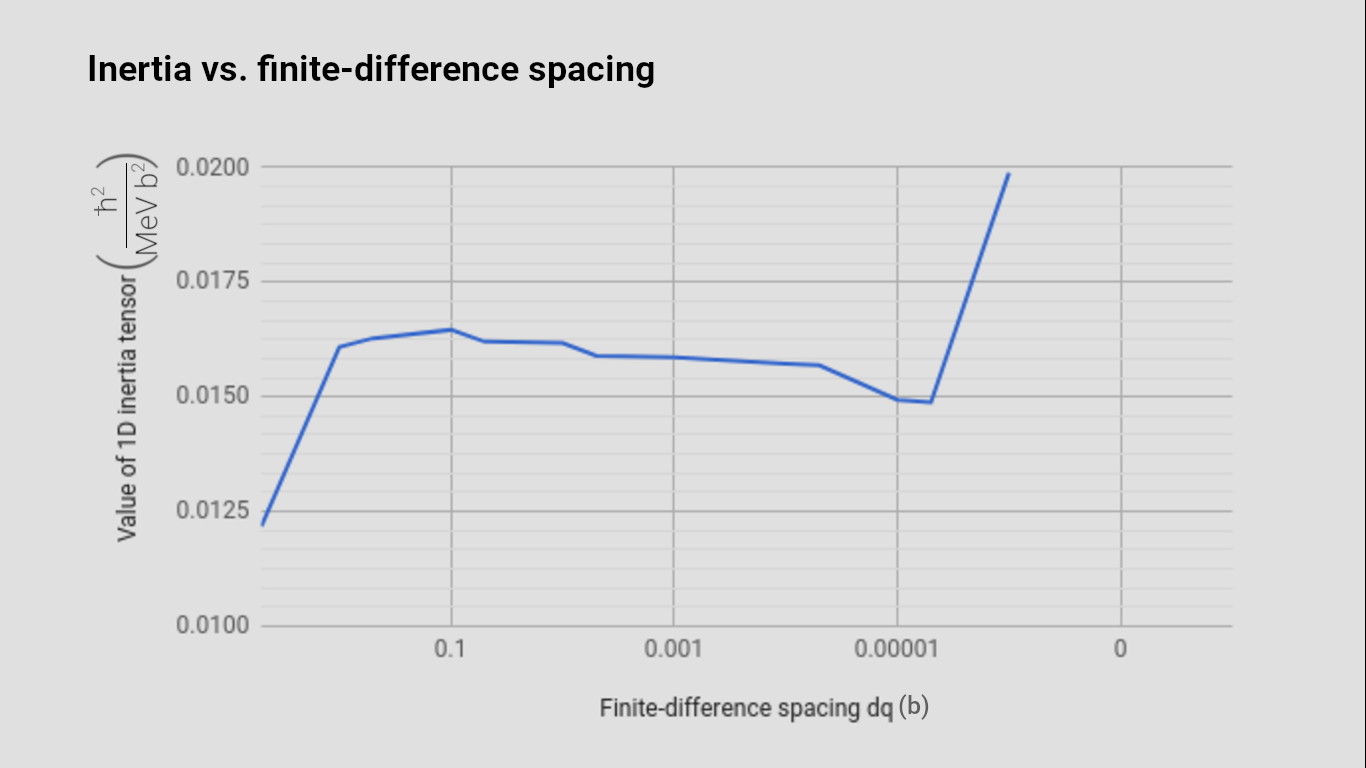
\includegraphics[width=0.7\linewidth]{TeX_files/Num-dq_spacing}
	\caption[Collective inertia as a function of finite-difference spacing]{$\mathcal{M}_{22}$ calculated for ??? configuration of $^{240}$Pu as a function of finite-difference spacing.}
	\label{fig:num-dqspacing}
\end{figure}

Figure \ref{fig:num-dqspacing} shows the effect of different values of $\delta q = \delta q'$ on the collective inertia for a particular configuration of $^{240}$Pu.

\begin{figure}
	\centering
	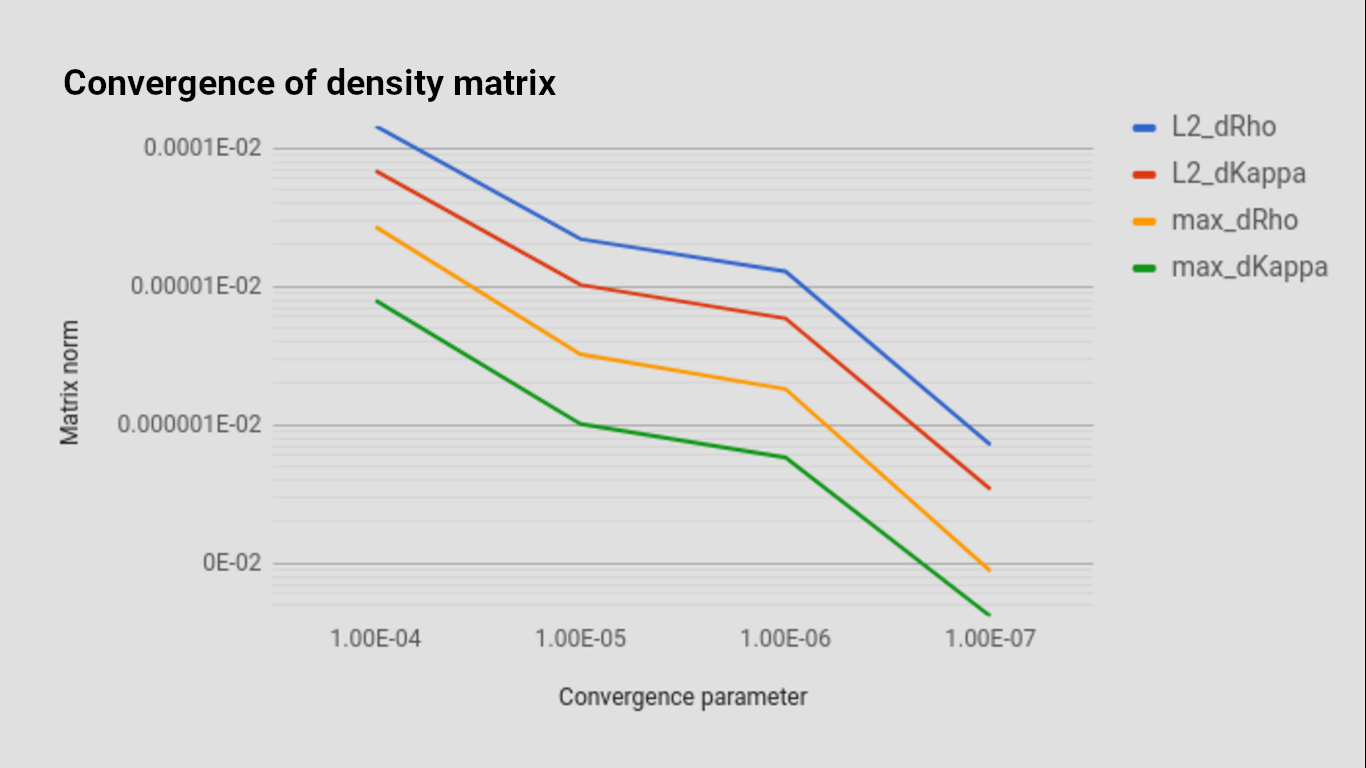
\includegraphics[width=0.7\linewidth]{TeX_files/Num-rho_conv}
	\caption[Norm of the difference matrix between subsequent iterations of the density]{Norm of the difference matrix between subsequent iterations of the density.}
	\label{fig:num-rhoconv}
\end{figure}

Figure \ref{fig:num-dqspacing} shows the norm of the matrix which corresponds to the difference between the density matrix at the last iteration and the second-to-last iteration. Predictably, the norm decreases as the convergence parameter becomes tighter. This gives a sense of the uncertainty associated with the density, which in turn should be propagated through equations \ref{eq:finite-diffs} and \ref{eq:mATDHFB-np}.

There are additional complications which arise in the finite-temperature formalism. These are discussed in Appendix \ref{append:TD-ATDHFB}.

\section{Minimum action path}
For tunneling through the barrier, the dynamic programming method \cite{Baran1981} was used. All DPM calculations for a particular Q20 can be performed in parallel, using OpenMP shared memory parallelism.

Were there any numerical issues associated with the minimum action path? We bumped it up to 4D, created continuation files. It is sensitive to $E_0$ still. We use the dynamic programming method to solve this part. That could be good to mention, although admittedly you're not the person who programmed it. There, the biggest issue is how large to set the search radius, which can strongly affect the total runtime, followed by how to keep it from going backwards. You also have to worry about interpolation.

Oh! You did add some basic parallelization. All DPM calculations for a particular Q20 can be performed in parallel, using OpenMP shared memory parallelism.

\section{Langevin}
And are there any numerical issues here, either? You need an interpolated surface, and the dynamics are carried out in discrete time steps. Can it be parallelized? Yes! I used MPI parallelism... For what part, exactly? Each outer turning point gets its own MPI rank. Why did I use MPI instead of OpenMP? I think it was to avoid a race condition when writing to a file? So now each rank gets its own? Or was it because of shared/private variables. How about this: ``I chose to use distributed-memory parallelism instead of shared-memory parallelism to simplify access to shared resources, such as variables and output files.''